\documentclass[journal]{IEEEtran}
\usepackage{lipsum} % 示例中使用的假文宏包
\usepackage{float}
\ifCLASSINFOpdf
\else
   \usepackage[dvips]{graphicx}
\fi
\usepackage{url}

\hyphenation{op-tical net-works semi-conduc-tor}
\usepackage{pdfpages} % 添加pdfpages宏包
\usepackage{graphicx}
\usepackage{xcolor}
\usepackage{wrapfig}
\usepackage{caption}
\usepackage{amsmath}
\begin{document}
\title{\color[rgb]{0,0.6,1}Digital Signal Processing Course Laboratory Experiments2 Report (October 2023)}

\author{12110405   Zhewei Chen}
%\thanks{This paragraph of the first footnote will contain the date on which you submitted your paper for review. It will also contain support information, including sponsor and financial support acknowledgment. For example, ``This work was supported in part by the U.S. Department of Commerce under Grant BS123456.'' }
%\thanks{The next few paragraphs should contain the authors' current affiliations, including current address and e-mail. For example, F. A. Author is with the National Institute of Standards and Technology, Boulder, CO 80305 USA (e-mail: author@boulder.nist.gov).}
%\thanks{S. B. Author, Jr., was with Rice University, Houston, TX 77005 USA. He is now with the Department of Physics, Colorado State University, Fort Collins, CO 80523 USA (e-mail: author@lamar.colostate.edu).}}

\markboth{EE323 Digital Signal Processing}
{Shell \MakeLowercase{\textit{et al.}}: Bare Demo of IEEEtran.cls for IEEE Journals}
\maketitle

\begin{abstract}
   This lab report introduces and investigates the basic concepts, representations and properties of discrete time systems. Using MATLAB to implement several discrete time systems and research their properties.
\end{abstract}

\begin{IEEEkeywords}
   discrete-time systems, difference equations, MATLAB
\end{IEEEkeywords}


\IEEEpeerreviewmaketitle



\section{Introduction}
\IEEEPARstart{T}{his} report is about Lab 2, focusing on the topic of discrete-time systems. The objective of the experiment is to learn the concepts and properties of discrete-time systems, understand the principles of discrete-time signal processing, and deepen the understanding of discrete-time systems through practical operation and analysis using MATLAB. We started by introducing the concept of discrete-time systems and discussed their importance and practical applications. We also analyzed the properties of discrete-time systems. In the background exercise section of the experiment, we designed integral and derivative discrete-time systems by selecting appropriate difference equations or block diagrams. We studied a difference equation case in the stock market. Next, we write MATLAB functions to implement integral and derivative discrete-time systems and study their properties. In the following stage, we design two types of discrete-time filters, test their impulse responses, and filter an audio signal. We then attempt to create the inverse system of one of the filters and validate it. Subsequently, we investigate the properties of the systems and perform comparative tests. Finally, we apply the filters to stock market data to analyze the properties.





\section{Experiment Contents}
\label{sec:guidelines}


\subsection{Breif Introduction of Discrete-Time Systems}

A discrete-time system takes discrete-time signals as input and produces discrete-time signals as output. It can simulate various scenarios, such as audio equalizer response or economic performance. Difference equations or block diagrams can represent discrete-time systems. Mathematically, we use the symbol $y = S(x)$ to denote a discrete-time system $S$ with input signal x[n] and output signal y[n]. They can be classified into categories such as linear/nonlinear, time-invariant/time-varying, causal/non-causal, memoryless/with memory, and stable/unstable.


\subsection{Background Exercises}
\subsubsection{Example Discrete-Time Systems}
Discrete-time digital systems are often used in place of analog processing systems. 
The following two continuous-time systems are commonly used in electrical engineering:
\vspace{\baselineskip}
\\differentiator: $ y(t) = \frac{d}{dt}x(t) $
\vspace{\baselineskip}
\\integrator: $ y(t) = \int\limits_{-\infty}^t x(\tau) d\tau $
\vspace{\baselineskip}

We can formulate discrete-time systems by replacing the differentiator and integrator with difference equations:
\vspace{\baselineskip}
\\differentiator:$~~y[n] = x[n] - x[n-1]$
\vspace{\baselineskip}
\\integrator:$~~y[n] = \sum_{k=-\infty}^{n} x[k]$

\vspace{\baselineskip}
Then writing down the difference equations of the two systems:
\vspace{\baselineskip}
\\differentiator:$~~y[n] = x[n] - x[n-1]$
\vspace{\baselineskip}
\\integrator:$~~y[n] = x[n] + y[n-1]$
\vspace{\baselineskip}

Finally drawing the block diagrams of the two systems:


\begin{figure}[H]
   \centering
   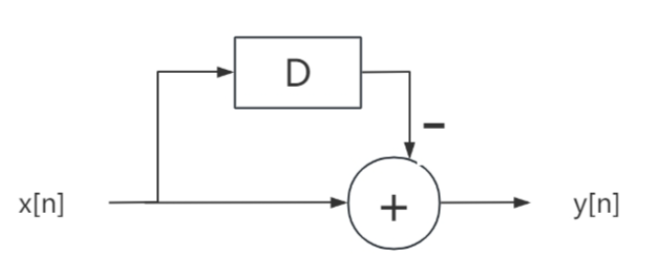
\includegraphics[width=0.45\textwidth]{differ.png} % 将"your_image.png"替换为您的PNG图片文件名
   \caption{Block diagram of differentiator }
   \label{fig:differ}
 \end{figure}

 \begin{figure}[H]
   \centering
   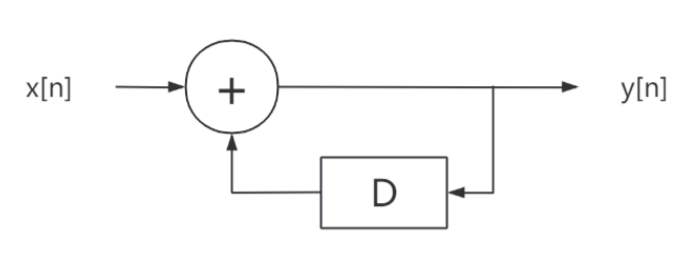
\includegraphics[width=0.5\textwidth]{integ.png} % 将"your_image.png"替换为您的PNG图片文件名
   \caption{Block diagram of integrator }
   \label{fig:integ}
 \end{figure}


\subsubsection{Stock Market Example}
The digital signal processing system can be used to analyze the signal in many cases. 
We try to apply DSP in a example in stock market.
One business magazine recommends three possible methods for computing the average value as follows:


\vspace{\baselineskip}
$\text{avgvalue[today]}$ = $\frac{1}{3} ( \text{value[today]} + \text{value[yesterday]} + \text{value[2 days ago]} ) $

\vspace{\baselineskip}
$\text{avgvalue[today]}$ =$ ~0.8 \cdot \text{avgvalue[yesterday]} + 0.2 \cdot \text{value[today]} $

\vspace{\baselineskip}
$\text{avgvalue[today]} $= $\text{avgvalue[yesterday]} + \frac{1}{3} (\text{value[today]} - \text{value[3 days ago]})$

\vspace{\baselineskip}
Then we can write the difference equations of the three methods:
 
\vspace{\baselineskip}
$y[n] = \frac{1}{3}(x[n]+x[n-1]+x[n-2])$ 
\vspace{\baselineskip}

$y[n] = 0.8y[n-1]+0.2x[n]$ 
\vspace{\baselineskip}

$y[n] = y[n-1]+\frac{1}{3}(x[n]-x[n-3])$

\vspace{\baselineskip}
Next,drawing the block diagrams of the three methods:
\begin{figure}[H]
   \centering
   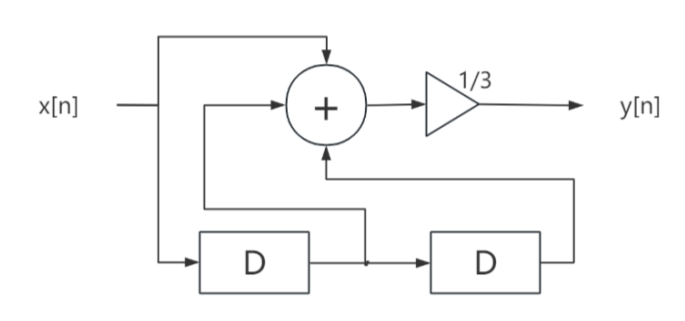
\includegraphics[width=0.5\textwidth]{2.2.1.png} % 将"your_image.png"替换为您的PNG图片文件名
   \caption{Block diagram of $y[n] = \frac{1}{3}(x[n]+x[n-1]+x[n-2])$  }
   \label{fig:2.2.1}
\end{figure}

\begin{figure}[H]
   \centering
   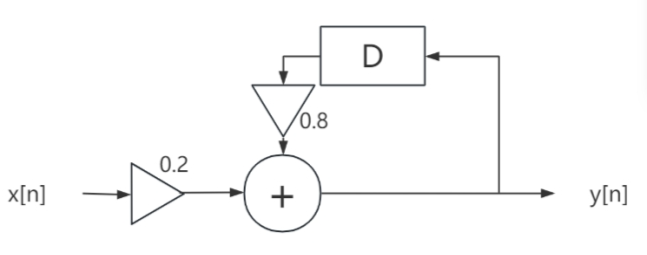
\includegraphics[width=0.5\textwidth]{2.2.2.png} % 将"your_image.png"替换为您的PNG图片文件名
   \caption{Block diagram of $y[n] = 0.8y[n-1]+0.2x[n]$ }
   \label{fig:2.2.2}
\end{figure}

\begin{figure}[H]
   \centering
   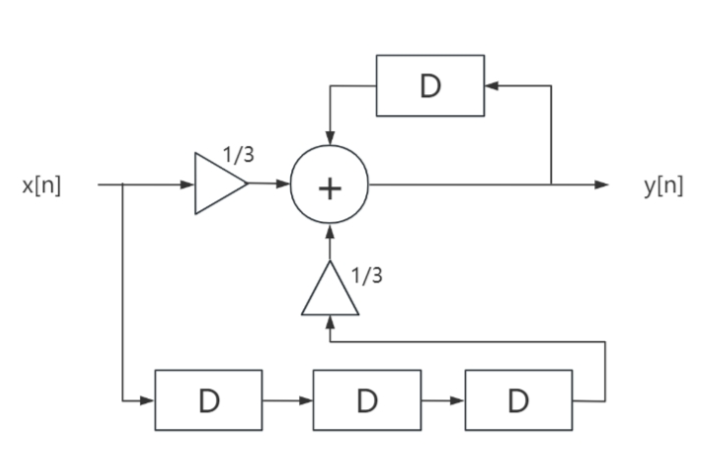
\includegraphics[width=0.5\textwidth]{2.2.3.png} % 将"your_image.png"替换为您的PNG图片文件名
   \caption{Block diagram of $y[n] = y[n-1]+\frac{1}{3}(x[n]-x[n-3])$ }
   \label{fig:2.2.3} 
\end{figure}
 

The impulse response of the three methods are shown below:
\begin{figure}[H]
   \centering
   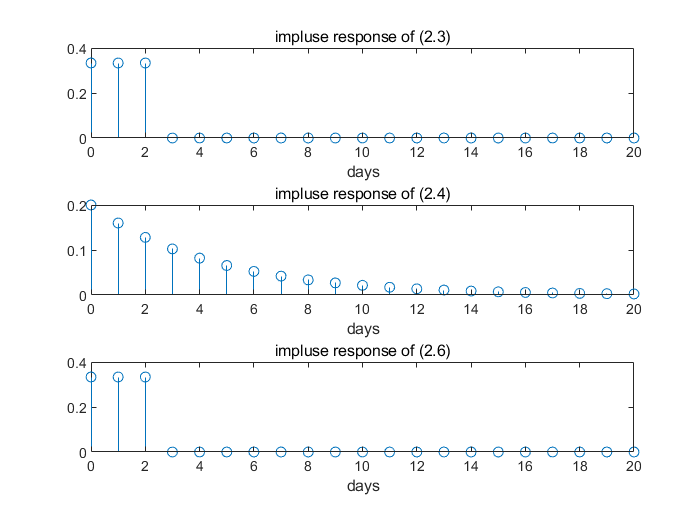
\includegraphics[width=0.5\textwidth]{2.2.png} % 将"your_image.png"替换为您的PNG图片文件名
   \caption{Impulse response of three methods   }
   \label{fig:2.2} 
\end{figure}
 
Method(2.3) and (2.5) is known as moving average method.

The method(2.3) difference equation $y[n] = \frac{1}{3}(x[n] + x[n-1] + x[n-2])$ represents the current output $y[n]$ as the average of the past three input signals $x[n]$, $x[n-1]$, and $x[n-2]$. This type of moving average method is called a three-point moving average because it uses three adjacent input samples for averaging.

The method(2.5) $y[n] = y[n-1] + \frac{1}{3}(x[n] - x[n-3])$ indicates that the current output $y[n]$ is the sum of the previous output $y[n-1]$ and the average of the difference between the current input $x[n]$ and the input from three steps ago $x[n-3]$, divided by 3. This type of moving average method is referred to as a three-point difference moving average because it involves averaging the difference between the current input and the input from three steps ago.

These two types of moving average methods can effectively smooth out noise in a signal and provide.



 %\begin{figure}[H]
  % \centering
   %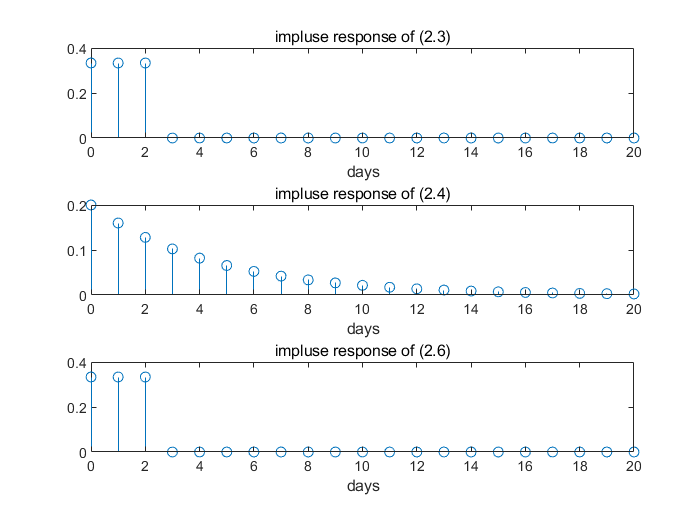
\includegraphics[width=0.5\textwidth]{2.2.png} % 将"your_image.png"替换为您的PNG图片文件名
   %\caption{bbox4 linearity test by inputs signal $x[n]=\delta[n]$ and $x[n]=u[n]$}
   %\label{fig:2.2}
 %\end{figure}

 


\subsection{Example Discrete-Time Systems}
Now we use MATLAB to implement the integrator and differentiator discrete-time systems. Then we set input signals $\delta[n]-\delta[n-5]$ and $\mu[n]-\mu[n-(N+1)], with N=10$ and to test the properties of the systems.
\begin{figure}[H]
   \centering
   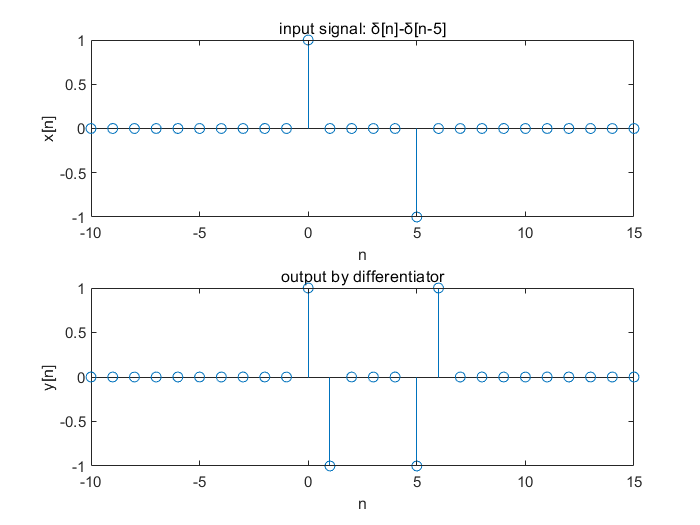
\includegraphics[width=0.4\textwidth]{2.3.1.png} % 将"your_image.png"替换为您的PNG图片文件名
   \caption{Test for differentiator system : when input signal is $\delta[n]-\delta[n-5]$}
   \label{fig:2.3.1} 
\end{figure}

\begin{figure}[H]
   \centering
   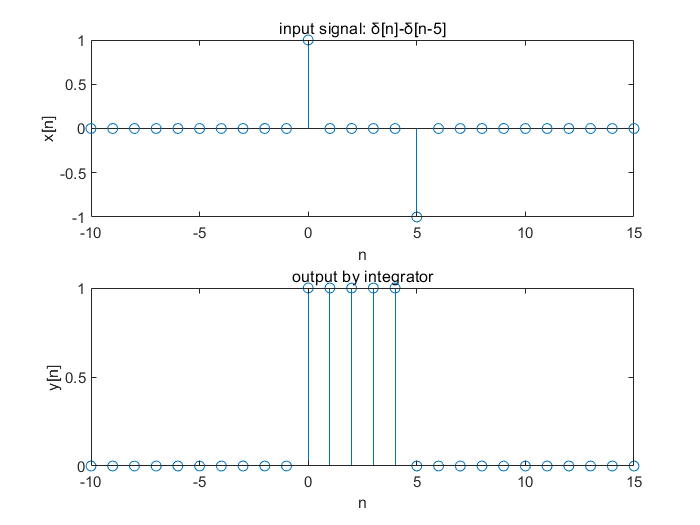
\includegraphics[width=0.4\textwidth]{2.3.2.png} % 将"your_image.png"替换为您的PNG图片文件名
   \caption{Test for integrator system : when input signal is $\delta[n]-\delta[n-5]$}
   \label{fig:2.3.2}
\end{figure}
\begin{figure}[H]
   \centering
   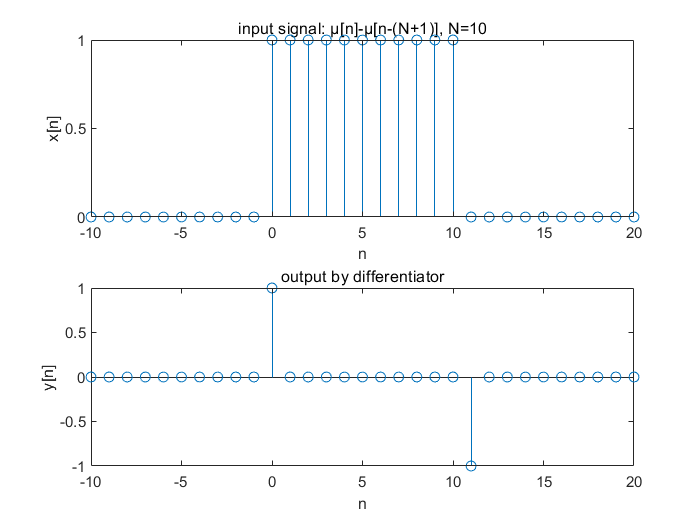
\includegraphics[width=0.4\textwidth]{2.3.3.png} % 将"your_image.png"替换为您的PNG图片文件名
   \caption{Test for differentiator system : when input signal is $\mu[n]-\mu[n-(N+1)], with N=10$}
   \label{fig:2.3.3}
\end{figure}
\begin{figure}[H]
   \centering
   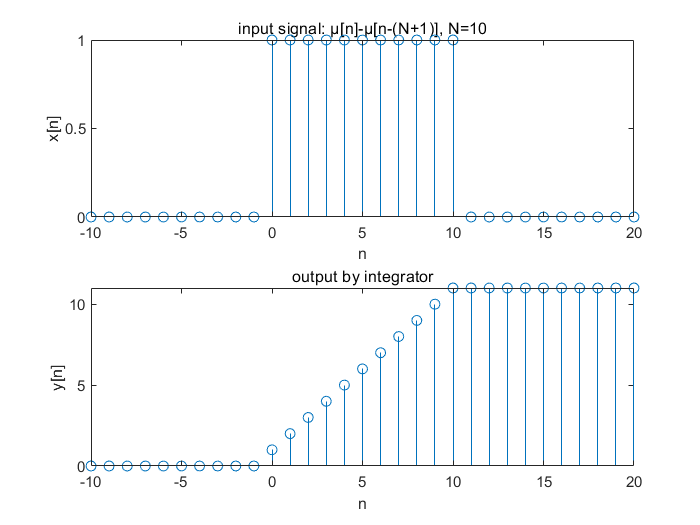
\includegraphics[width=0.4\textwidth]{2.3.4.png} % 将"your_image.png"替换为您的PNG图片文件名
   \caption{Test for integrator system : when input signal is $\mu[n]-\mu[n-(N+1)], with N=10$}
   \label{fig:2.3.4}
\end{figure}

Stability:
\subsubsection{differentiator} $y[n]=x[n]-x[n-1]$, is BIBO bounded, because when $x[n]$ is bounded, $x[n]-x[n-1](y[n])$ is also bounded.
\subsubsection{integrator} $y[n]=x[n]+y[n-1]$, is NOT BIBO bounded.When we set input signal $x[n]=\mu[n]$, the output signal contains increaes when n increaes.(Also we may apply Z-transform to check the stability of system, waiting for further progress in the course)
\subsection{Difference Equations}
After trying two simple examples of discrete-time systems,we will study the effort of two filters. 
\\The difference equations of the two filters are shown below:

\vspace{\baselineskip}
$y=S_{1}(x)$  :      $y[n]=x[n]-x[n-1]$ 

\vspace{\baselineskip}
$y=S_{2}(x)$ : $y[n]=x[n]+\frac{1}{2}y[n-1]$

\vspace{\baselineskip}

Now we use system diagram and set input signal as $\delta[n]$ calculate the impulse response of the five systems :
$y=S_{1}(x)$,$~$$y=S_{2}(x)$,$~$$y=S_{1}(S_{2}(x))$,$~$$y=S_{2}(S_{1}(x))$,$~$$y=S_{1}(x)+S_{2}(x)$

($y=S_{1}(S_{2}(x))$ and $y=S_{2}(S_{1}(x))$ actually means series connection in bolck diagrams)

System Diagram and Impulse Response:
\begin{figure}[H]
   \centering
   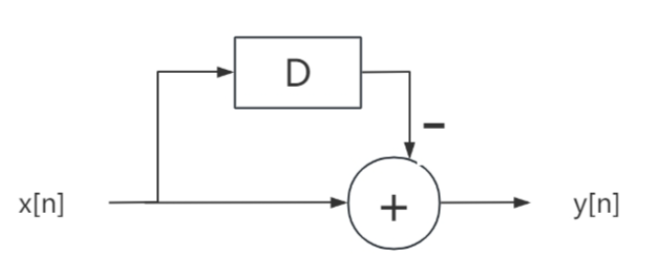
\includegraphics[width=0.5\textwidth]{differ.png} % 将"your_image.png"替换为您的PNG图片文件名
   \caption{Block Diagram of system : $y=S_{1}(x)$}
   \label{fig:differ2} 
\end{figure}
\begin{figure}[H]
   \centering
   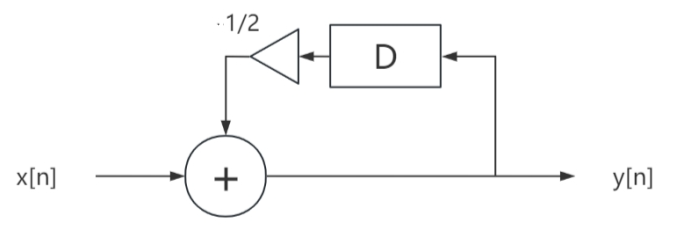
\includegraphics[width=0.5\textwidth]{S2.png} % 将"your_image.png"替换为您的PNG图片文件名
   \caption{Block Diagram of system : $y=S_{2}(x)$}
   \label{fig:S12} 
\end{figure}
\begin{figure}[H]
   \centering
   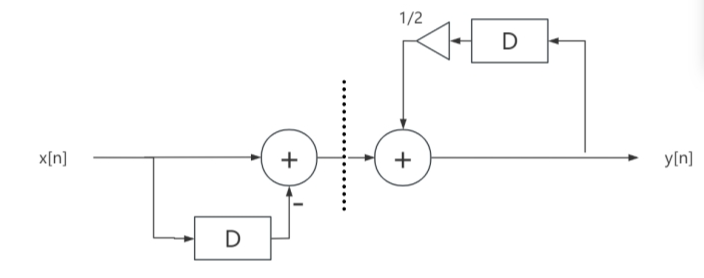
\includegraphics[width=0.5\textwidth]{S12.png} % 将"your_image.png"替换为您的PNG图片文件名
   \caption{Block Diagram of system : $y=S_{1}(S_{2}(x))$} 
   \label{fig:S12} 
\end{figure}
\begin{figure}[H]
   \centering
   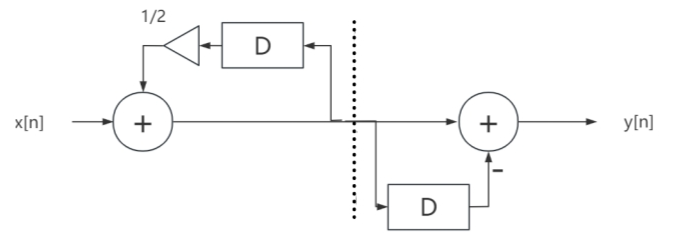
\includegraphics[width=0.5\textwidth]{S21.png} % 将"your_image.png"替换为您的PNG图片文件名
   \caption{Block Diagram of system : $y=S_{2}(S_{1}(x))$} 
   \label{fig:S21} 
\end{figure}
\begin{figure}[H]
   \centering
   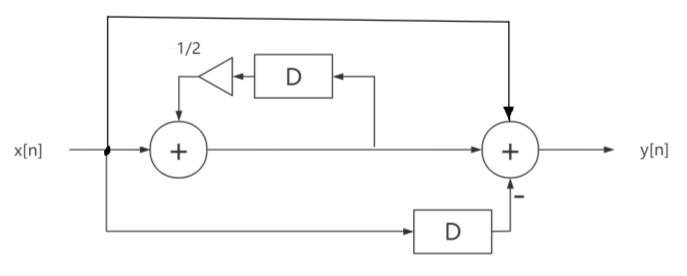
\includegraphics[width=0.5\textwidth]{S1S2.png} % 将"your_image.png"替换为您的PNG图片文件名
   \caption{Block Diagram of system : $y=S_{1}(x)+S_{2}(x)$}
   \label{fig:S1S2} 
\end{figure}



\begin{figure}[H]
   \centering
   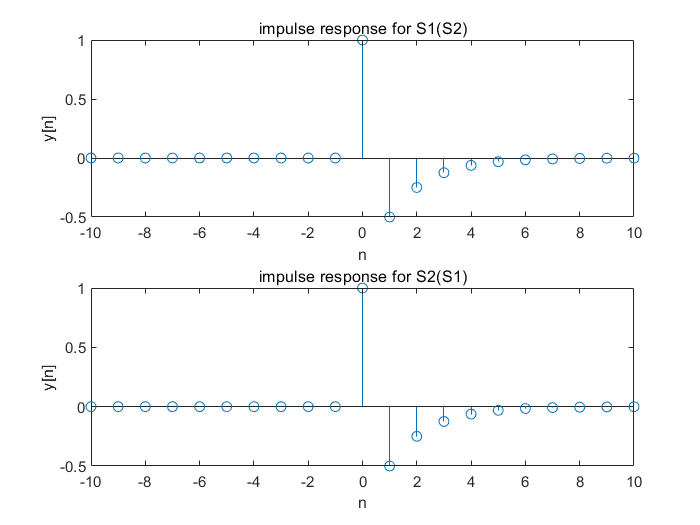
\includegraphics[width=0.5\textwidth]{2.4.2.png} % 将"your_image.png"替换为您的PNG图片文件名
   \caption{Impulse response of systems $y=S_{1}(S_{2}(x))$ and $y=S_{2}(S_{1}(x))$   }
   \label{fig:2.4.2} 
\end{figure}

\begin{figure}[H]
   \centering
   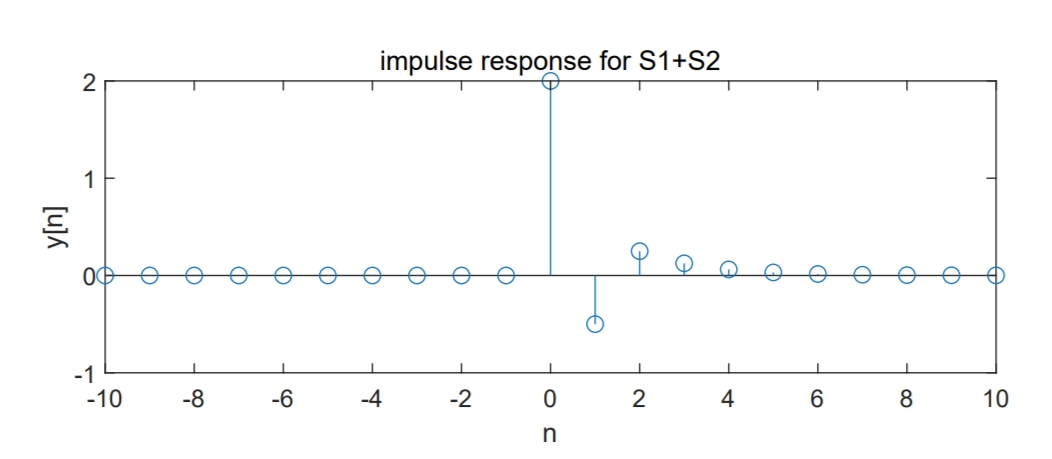
\includegraphics[width=0.5\textwidth]{2.4.3.png} % 将"your_image.png"替换为您的PNG图片文件名
   \caption{Impulse response of system : $y=S_{1}(x)+S_{2}(x)$ }
   \label{fig:2.4.3} 
\end{figure}

Note that the impulse response of $y=S_{1}(S_{2}(x))$ and $y=S_{2}(S_{1}(x))$ are the same, which means that the two systems are equivalent and series connection of the two systems is commutative.

$y=S_{1}(x)+S_{2}(x)$is parallel connection, the output is equal to the sum of individual outputs, and they do not interfere with each other,according to the plot of impulse responses.

\subsection{Audio Filtering}
In this section, we will use the two filters designed in the previous section to filter an audio signal to test the effect of them.

After filtering and play the sound, we found that human ears could only perceive a reduction in background music when listening to the sound filtered through S1. The sound filtered through S2 and the original sound had a subtle distinction that couldn't be precisely described.

To get further difference between the sound after filtering and the original sound, we use MATLAB to plot the spectrums and waveforms of the sound before and after filtering. 

The spectrum of the original sound is shown below:

\begin{figure}[H]
   \centering
   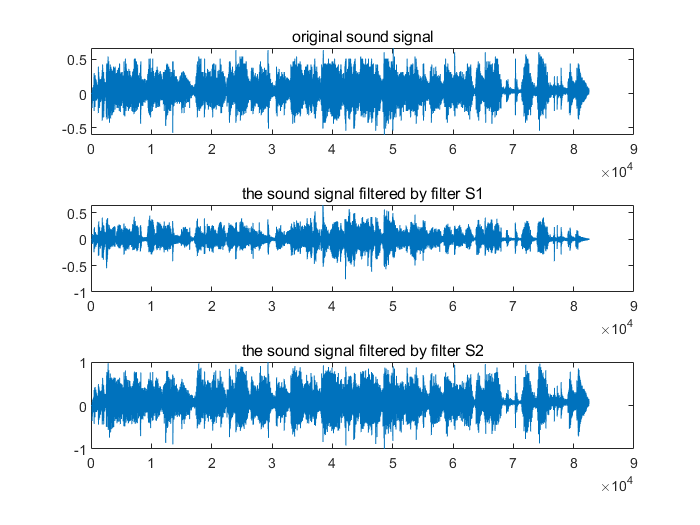
\includegraphics[width=0.5\textwidth]{2.5.1.png} % 将"your_image.png"替换为您的PNG图片文件名
   \caption{Waveforms of the sound before and after filtering}
   \label{fig:2.5.1}
\end{figure}

\begin{figure}[H]
   \centering
   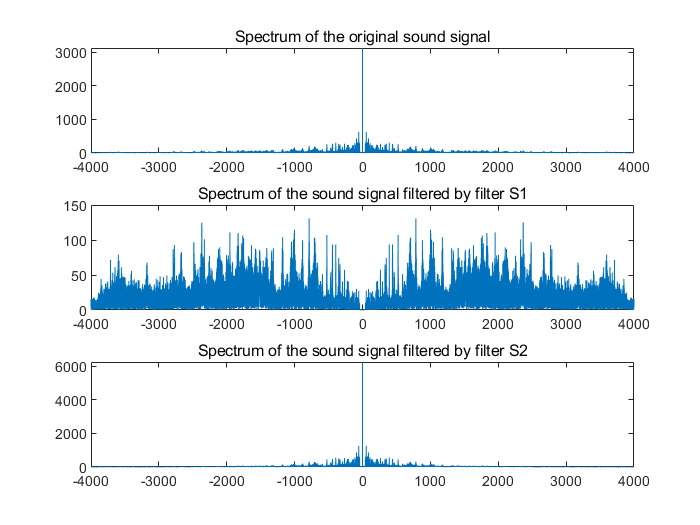
\includegraphics[width=0.5\textwidth]{2.5.2.png} % 将"your_image.png"替换为您的PNG图片文件名
   \caption{Spectrums of the sound before and after filtering}
   \label{fig:2.5.2}
\end{figure}

In the waveform, the signal filtered by the $S_{1}$ filter shows a significant decrease in overall amplitude, and in the spectrum, the low-frequency (around zero) signals are nearly eliminated. On the other hand, 
the signal filtered by the $S_{2}$ filter exhibits minimal differences compared to the original signal.


\subsection{Inverse Systems}
In this section, we will try to design the inverse system $(y=S_{3}(x))$ of $y=S_{2}(x)$ and validate it.
Assume that $\delta = S_{3}(S_{2}(x))$ where $\delta$ denotes the discrete-time impulse function $\delta [n]$. Since both systems $S_{2}(x)$ and $S_{3}(x)$ are LTI, the time-invariance and superposition properties can be used to obtain $x = S_{3}(S_{2}(x))$ for any discrete-time signal $x$. We say that the systems $S_{3}(x)$ and $S_{2}(x)$ are inverse filters because 
they cancel out the effects of each other. 
According to the Hint, because $S_{2}(x)$ : $y[n]=x[n]+\frac{1}{2}y[n-1]$we can write the difference equation 
of $S_{3}(x)$ as follows:$~~~$$x[n]=y[n]+\frac{1}{2}x[n-1]$
(simply exchange x,y) 

\begin{figure}[H]
   \centering
   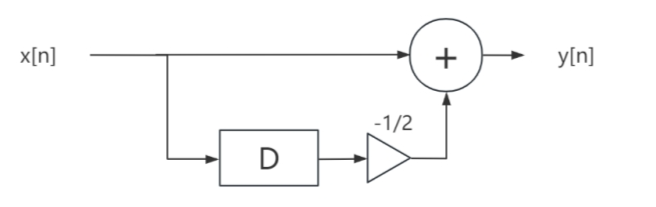
\includegraphics[width=0.5\textwidth]{S3.png} % 将"your_image.png"替换为您的PNG图片文件名
   \caption{Block Diagram of system : $y=S_{3}(x)$}
   \label{fig:S3} 
\end{figure}
\begin{figure}[H]
   \centering
   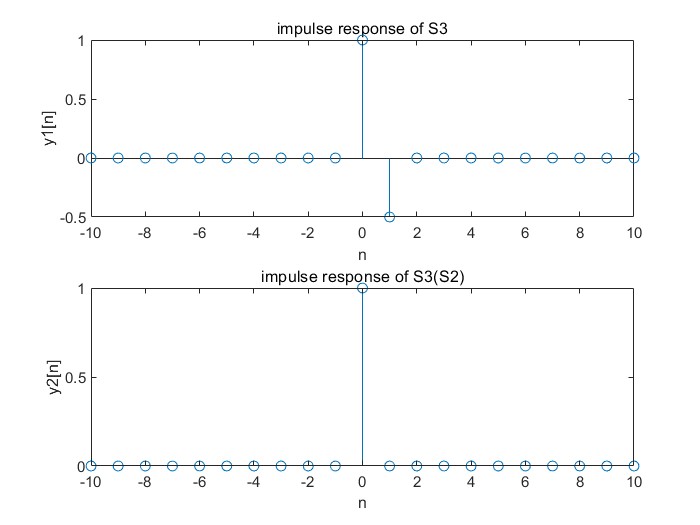
\includegraphics[width=0.45\textwidth]{2.6.png} % 将"your_image.png"替换为您的PNG图片文件名
   \caption{Impulse response of $y=S_{3}(x)$ and $y=S_{3}(S_{2}(x))$}
   \label{fig:2.6}
\end{figure}

As the plot shows, the systems $S_{3}(x)$ and $S_{2}(x)$ are inverse filters because the impulse response of $y=S_{3}(S_{2}(x))$ is $\delta$.

\subsection{Systems Tests}
Discrete-time systems have many properties, such as linearity, time-invariance, causality, stability, and invertibility. In this section, we will test linearity and time-invariance of three systems $y=bboxN(x)$ where $N=4,5,6$.


\begin{figure}[H]
   \centering
   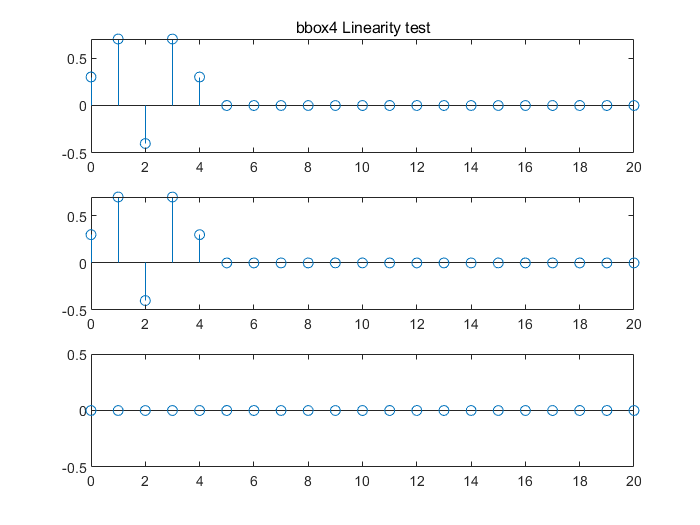
\includegraphics[width=0.45\textwidth]{2.7.1.png} % 将"your_image.png"替换为您的PNG图片文件名
   \caption{bbox4 linearity test by inputs signal $x[n]=\delta[n]$ and $x[n]=2\delta[n]$}
   \label{fig:2.7.1}
\end{figure}
\begin{figure}[H]
   \centering
   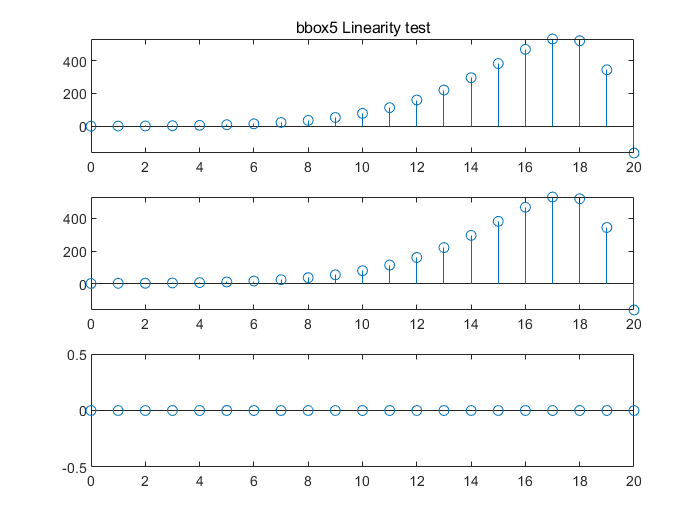
\includegraphics[width=0.45\textwidth]{2.7.2.png} % 将"your_image.png"替换为您的PNG图片文件名
   \caption{bbox5 linearity test by inputs signal $x[n]=\delta[n]$ and $x[n]=2\delta[n]$}
   \label{fig:2.7.2}
\end{figure}
\begin{figure}[H]
   \centering
   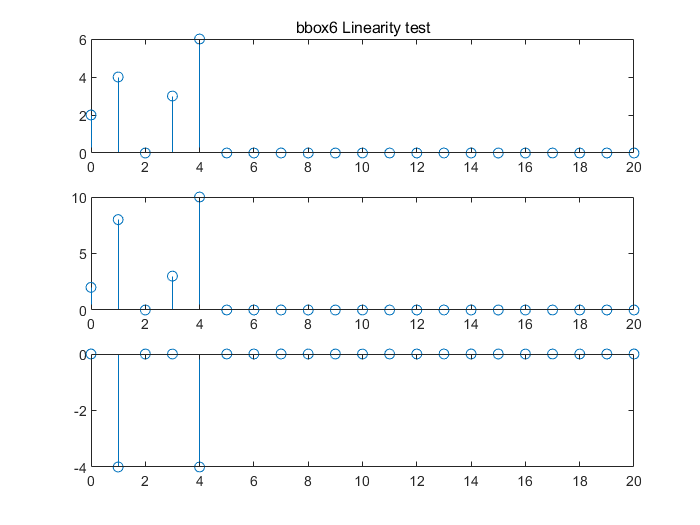
\includegraphics[width=0.45\textwidth]{2.7.3.png} % 将"your_image.png"替换为您的PNG图片文件名
   \caption{bbox6 linearity test by inputs signal $x[n]=\delta[n]$ and $x[n]=2\delta[n]$}
   \label{fig:2.7.3}
\end{figure}
\begin{figure}[H]
   \centering
   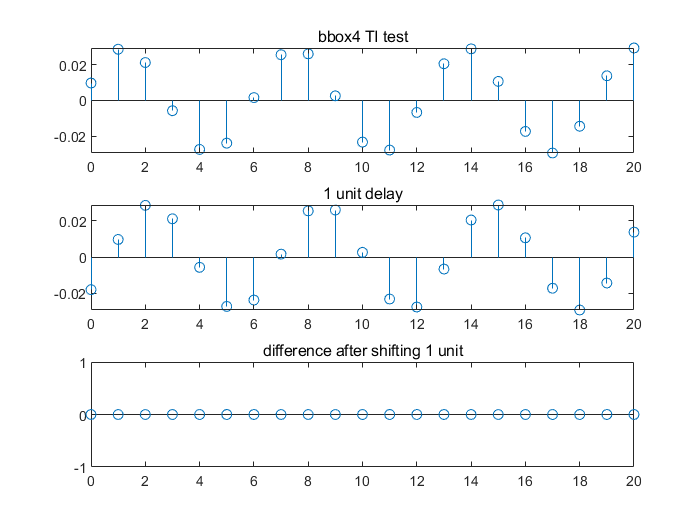
\includegraphics[width=0.45\textwidth]{2.7.4.png} % 将"your_image.png"替换为您的PNG图片文件名
   \caption{bbox4 time-invariance test by inputs signal $x[n]=cos(n)$ and $x[n]=cos(n-1)$}
   \label{fig:2.7.4}
\end{figure}
\begin{figure}[H]
   \centering
   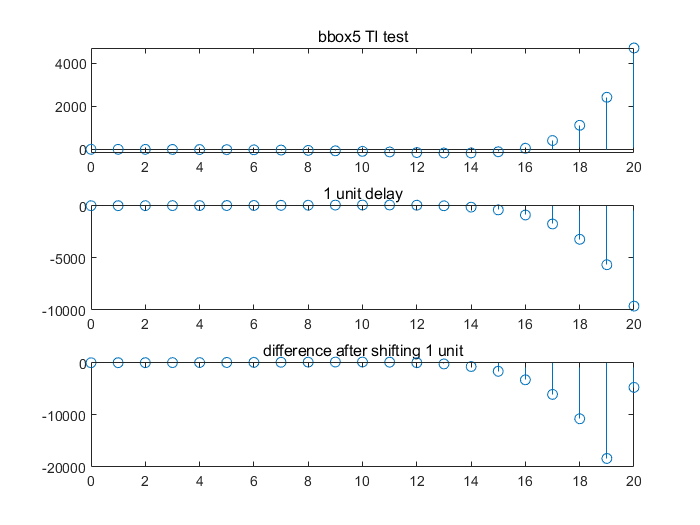
\includegraphics[width=0.48\textwidth]{2.7.5.png} % 将"your_image.png"替换为您的PNG图片文件名
   \caption{bbox4 time-invariance test by inputs signal $x[n]=cos(n)$ and $x[n]=cos(n-1)$}
   \label{fig:2.7.5}
\end{figure}

\begin{figure}[H]
   \centering
   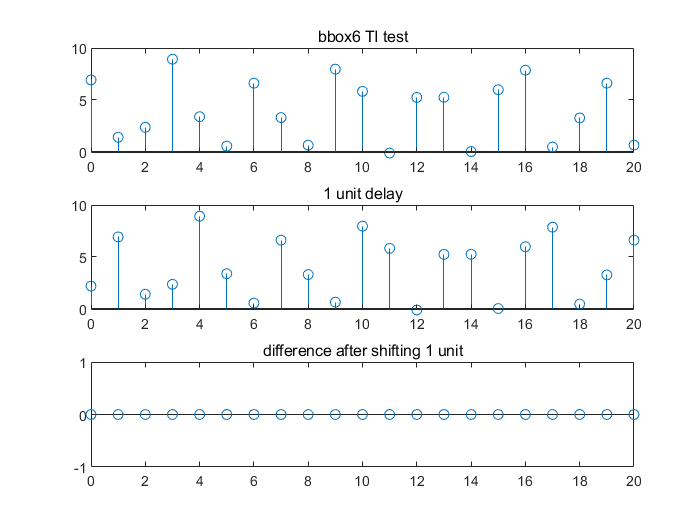
\includegraphics[width=0.48\textwidth]{2.7.6.png} % 将"your_image.png"替换为您的PNG图片文件名
   \caption{bbox4 time-invariance test by inputs signal $x[n]=cos(n)$ and $x[n]=cos(n-1)$}
   \label{fig:2.7.6}
\end{figure}

Because of the inability to make judgments based on the response obtained from an impulse function input, 
we utilized the cosine function input instead. 

Based on the Fig.24, the result of $bbox6(\delta[n])+2*bbox6(\delta[n-1])-bbox6(2\delta[n-1]+\delta[n])$ is not zero, 
it can be observed that the only \textbf{non-linear system is bbox6}.

Based on the Fig.26 the only time-varying system is bbox5. We do subtraction between the two outputs of bbox5 (including shifting 1 unit) and the result is not zero.

\subsection{Stock Market Example}
After studying the concepts and properties of discrete-time systems, we attempt to use filters to investigate a practical example.
We will utilize filters 1 and 2 to smooth out these stock values. 
It is necessary to initialize filters  and  with a value of zero.

\begin{figure}[H]
   \centering
   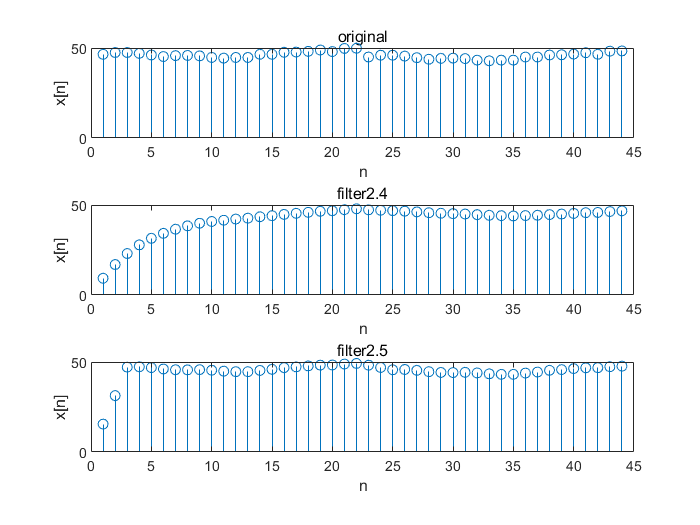
\includegraphics[width=0.5\textwidth]{2.8.png} % 将"your_image.png"替换为您的PNG图片文件名
   \caption{Spectrums of the sound before and after filtering}
   \label{fig:2.8}
\end{figure}
\subsubsection{}Disadvantage and advantage of the two filters



The signal filtered by filter (2.4) appears smoother, but it deviates significantly from the original signal over a longer duration. On the other hand, filter (2.5) achieves output that resembles the original signal more quickly, but it introduces step-like transitions  in the filtered signal at the beginning.

\subsubsection{}Initialize the filters outputs

Maintaining consistency between the initial outputs and inputs yields better results in obtaining the desired output.

\section{Conclusion}

Through this experiment, we have reached the following conclusions: 

Discrete-time systems are highly useful mathematical tools that can be applied in various fields for signal processing. Different systems (filters) are suitable for different situations. In practical scenarios, it is advisable to start with mathematical modeling to obtain an approximate representation using difference equations. We can describe systems through mathematical expressions (including difference equations), system block diagrams, and programming languages to provide multiple perspectives.

For systems with known difference equations, we can make initial conjectures about their properties and then use MATLAB or other tools to test these properties. However, for systems with completely unknown internal mathematical relationships, we can only rely on tools like MATLAB to exclude possibilities. For example, analyzing the system's output for specific inputs can help determine whether it is time-invariant, such as the case of bbox5. 

It is important to note that in practical situations, the parameters or design of filters may need to be optimized to meet specific requirements. 
Additionally, different output methods may not provide definitive conclusions. 
For instance, relying solely on auditory perception in audio filtering may not effectively indicate the results, and using only impulse functions as inputs in time invariance tests may not yield conclusive results. Therefore, it is best to employ multiple methods and perform multiple validations using different inputs to obtain reliable results.



\end{document}
